\documentclass{beamer}
\usetheme{Boadilla}

\title{Parity Asymmetry in the CMB}
\subtitle{UF REU under Dr. Zachary Slepian}
\author{Michael Bartlett}
\institute{University of Oklahoma}
\date{\today}

\begin{document}

\begin{frame}
    \titlepage
\end{frame}

\begin{frame}
    \frametitle{Outline}
    \tableofcontents
\end{frame}

\section{Overview of the Problem}

\section{Initial Calculations}
    \begin{frame}
        \frametitle{Intitial Calculations}
        Start by expanding the two correlation functions in terms of isotropic basis functions:
        \begin{eqnarray*}
            \zeta_{x_0} (\vec r_1, \vec r_2, \vec r_3) &=& \sum_{\Lambda} \tilde{\zeta_{\Lambda}}(r_1, r_2, r_3) \mathcal P_{\Lambda}(\hat r_1, \hat r_2, \hat r_3)\\
            \zeta_E (\vec x_0, \vec x_1, \vec x_2, \vec x_3) &=& \sum_{\Lambda '} \tilde{\zeta_{\Lambda '}}(x_0, x_1, x_2, x_3) \mathcal P_{\Lambda '}(\hat x_0, \hat x_1, \hat x_2, \hat x_3)
        \end{eqnarray*}
        Where $\Lambda$ is the set $\{l_1, l_2, l_3\}$ and $\Lambda'$ is the set $\{l_0', l_1', l_{01}', l_2', l_3'\}$
    \end{frame}

    \begin{frame}
        \frametitle{Intitial Calculations}
        We can then set the two functions equal since they are correlation functions describing the same points
        \begin{eqnarray*}
            \zeta_{x_0} (\vec r_1, \vec r_2, \vec r_3) &=& \zeta_E (\vec x_0, \vec x_1, \vec x_2, \vec x_3)\\
            &\Downarrow&\\
            \sum_{\Lambda} \zeta_{\Lambda}(r_1, r_2, r_3) \mathcal P_{\Lambda}(\hat r_1, \hat r_2, \hat r_3) &=& \sum_{\Lambda '} \zeta_{\Lambda '}(x_0, x_1, x_2, x_3) \mathcal P_{\Lambda '}(\hat x_0, \hat x_1, \hat x_2, \hat x_3)
        \end{eqnarray*}
    \end{frame}

    \begin{frame}
        \frametitle{Intitial Calculations}
        We now multiply both sides by $\mathcal P_{\Lambda ''}^*(\hat x_0, \hat x_1, \hat x_2, \hat x_3)$ and then integrate over all orientations
        $d \hat x_0 d \hat x_1 d \hat x_2 d \hat x_3 = d \hat x$
        \begin{eqnarray*}
            \int d \hat x \sum_{\Lambda} \zeta_{\Lambda}(r_1, r_2, r_3) \mathcal P_{\Lambda}(\hat r_1, \hat r_2, \hat r_3) P^*_{\Lambda ''}(\hat x_0, \hat x_1, \hat x_2, \hat x_3) = \\
            \int d \hat x \sum_{\Lambda '} \zeta_{\Lambda '}(x_0, x_1, x_2, x_3) \mathcal P_{\Lambda '}(\hat x_0, \hat x_1, \hat x_2, \hat x_3) P^*_{\Lambda ''}(\hat x_0, \hat x_1, \hat x_2, \hat x_3)
        \end{eqnarray*}
    \end{frame}

    \begin{frame}
        \frametitle{Intitial Calculations}
        Using the orthogonality of isotropic basis functions which states\\
        $$\int d \hat R \ \mathcal P_{\Lambda}(\hat R) \mathcal P^*_{\Lambda'}(\hat R) = \delta_{\Lambda_1 \Lambda_1'}\delta_{\Lambda_2 \Lambda_2'}...$$\\
        we can simplify the right hand side of the previous equation:
        \begin{multline*}
            \int d \hat x \sum_{\Lambda '} \zeta_{\Lambda '}(x_0, x_1, x_2, x_3) \mathcal P_{\Lambda '}(\hat x_0, \hat x_1, \hat x_2, \hat x_3) P_{\Lambda ''}(\hat x_0, \hat x_1, \hat x_2, \hat x_3)\\
            =\zeta_{\Lambda ''}(x_0, x_1, x_2, x_3)
        \end{multline*}
    \end{frame}

    \begin{frame}
        \frametitle{Intitial Calculations}
        Plugging this back into the previous equation we get the key relation:
        \begin{equation}
        \boxed{\zeta_{\Lambda ''}(x_0, x_1, x_2, x_3) = \int d \hat x \sum_{\Lambda} \zeta_{\Lambda}(r_1, r_2, r_3) \mathcal P_{\Lambda}(\hat r_1, \hat r_2, \hat r_3) P^*_{\Lambda ''}(\hat x_0, \hat x_1, \hat x_2, \hat x_3)}
        \end{equation}
        Solving the integral on the right will
        give an expression for the coefficients of the correlation function centered 
        on earth in terms of the correlation function centered at $x_0$
    \end{frame}

    \begin{frame}
        \frametitle{Solving for $\vec r$ in terms of $\vec x$}
        Consider a great circle going through the poles at an angle $\phi_i$ to the x-axis where
        $\phi_i$ is the $\phi$ angle of vector $\vec x_i$ for $i = 1,2,3$\\
        \begin{figure}
            \centering
                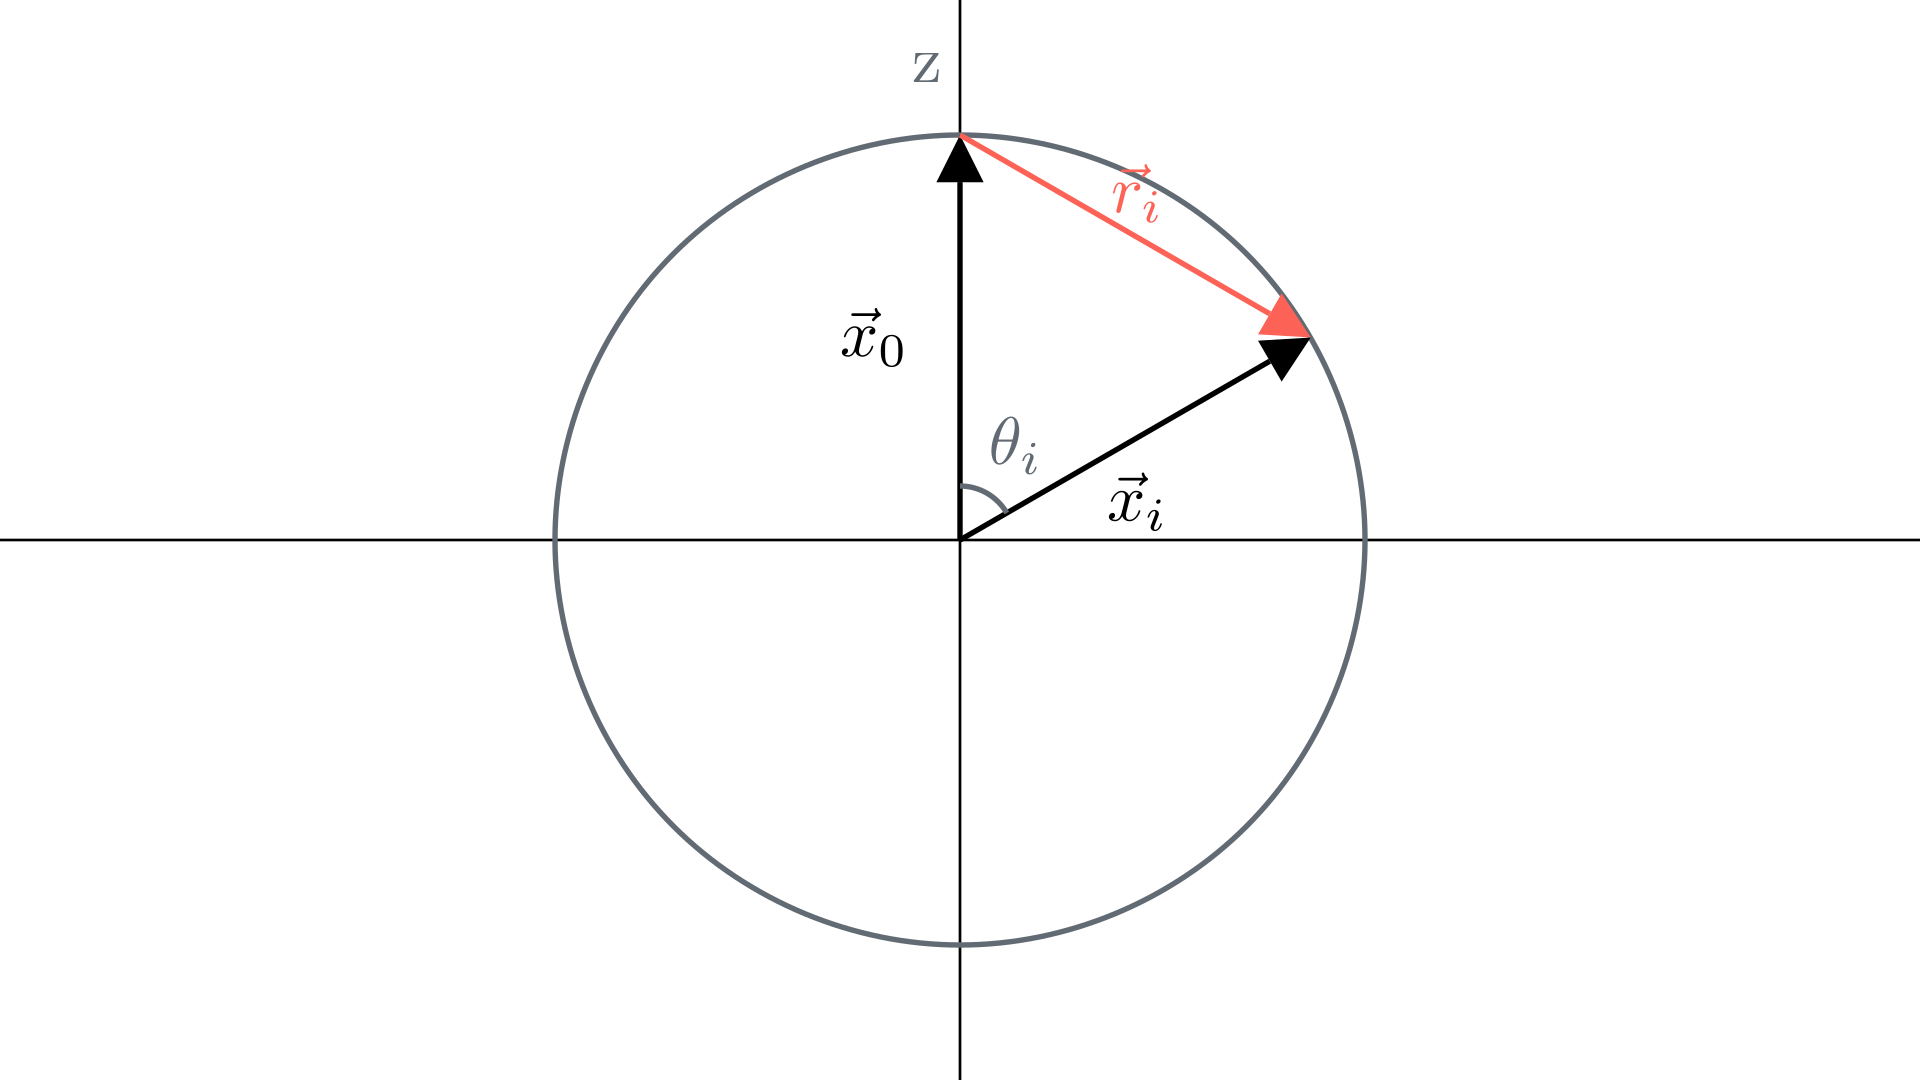
\includegraphics[width=1\textwidth]{media/angle_conversion_diagram_2_ManimCE_v0.17.3.png}
            \end{figure}
    \end{frame}

    \begin{frame}
        \frametitle{Solving for $\vec r$ in terms of $\vec x$}
        Using the law of Cosines and defining the distance to the cmb to be $d^*$ we get:\\
        \begin{equation*}
            |\vec r_i| = \sqrt{d^{*2} + d^{*2} - 2d^*d^*cos(\theta_i)}
        \end{equation*}
        \begin{equation*}
            \boxed{r_i = \sqrt{2}d^*\sqrt{1 - cos(\theta_i)}}
        \end{equation*}

        \begin{figure}
            \centering
                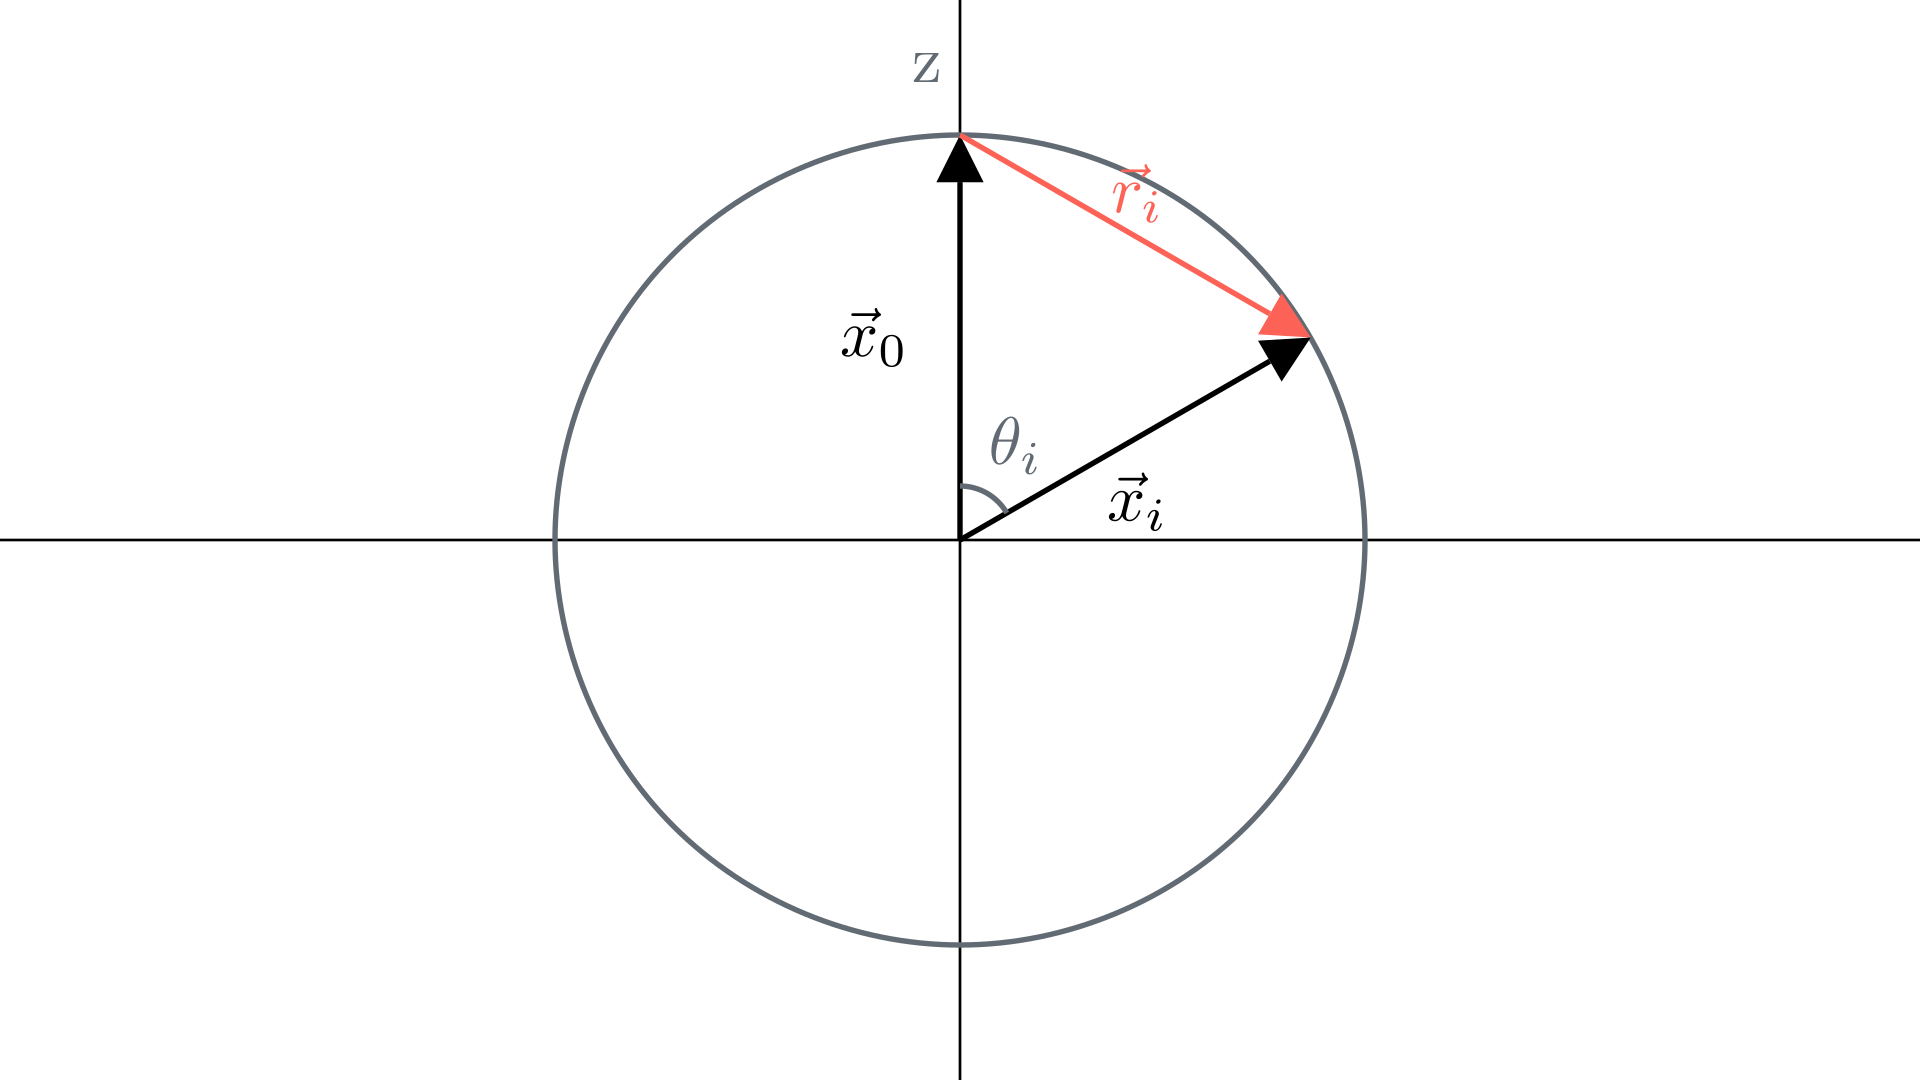
\includegraphics[width=0.8\textwidth]{media/angle_conversion_diagram_2_ManimCE_v0.17.3.png}
            \end{figure}
    \end{frame}

\section{Solving for Coefficients}



\end{document}
